\section{Perceptron}

In the 1940s, computers were already proficient at executing tasks exactly as programmed and performing arithmetic operations with impressive speed. 
However, researchers envisioned machines that could do much more. 
They wanted computers that could handle noisy data, interact directly with their environment, function in a massively parallel and fault-tolerant way, and adapt to changing circumstances. 
Their quest was for a new computational model, one that could surpass the constraints of the Von Neumann Machine.

\subsection{Human neurons}
The human brain contains an enormous number of computing units, with approximately 100 billion neurons, each connected to around 7,000 other neurons through synapses. 
In adults, this results in a total of 100 to 500 trillion synaptic connections, while in a three-year-old child, this number can reach up to 1 quadrillion synapses.

The brain's computational model is characterized by its distributed nature among simple, non-linear units, its redundancy which ensures fault tolerance, and its intrinsic parallelism. 
The perceptron, a computational model inspired by the brain, reflects these principles.

Information in the brain is transmitted through chemical processes. 
Dendrites gather signals from synapses, which can be either inhibitory or excitatory.
When the cumulative charge reaches a certain threshold, the neuron fires, releasing the charge.

\subsection{Artificial neuron}
The mathematical model of a neuron is represented as follows:
\begin{figure}[H]
    \centering
    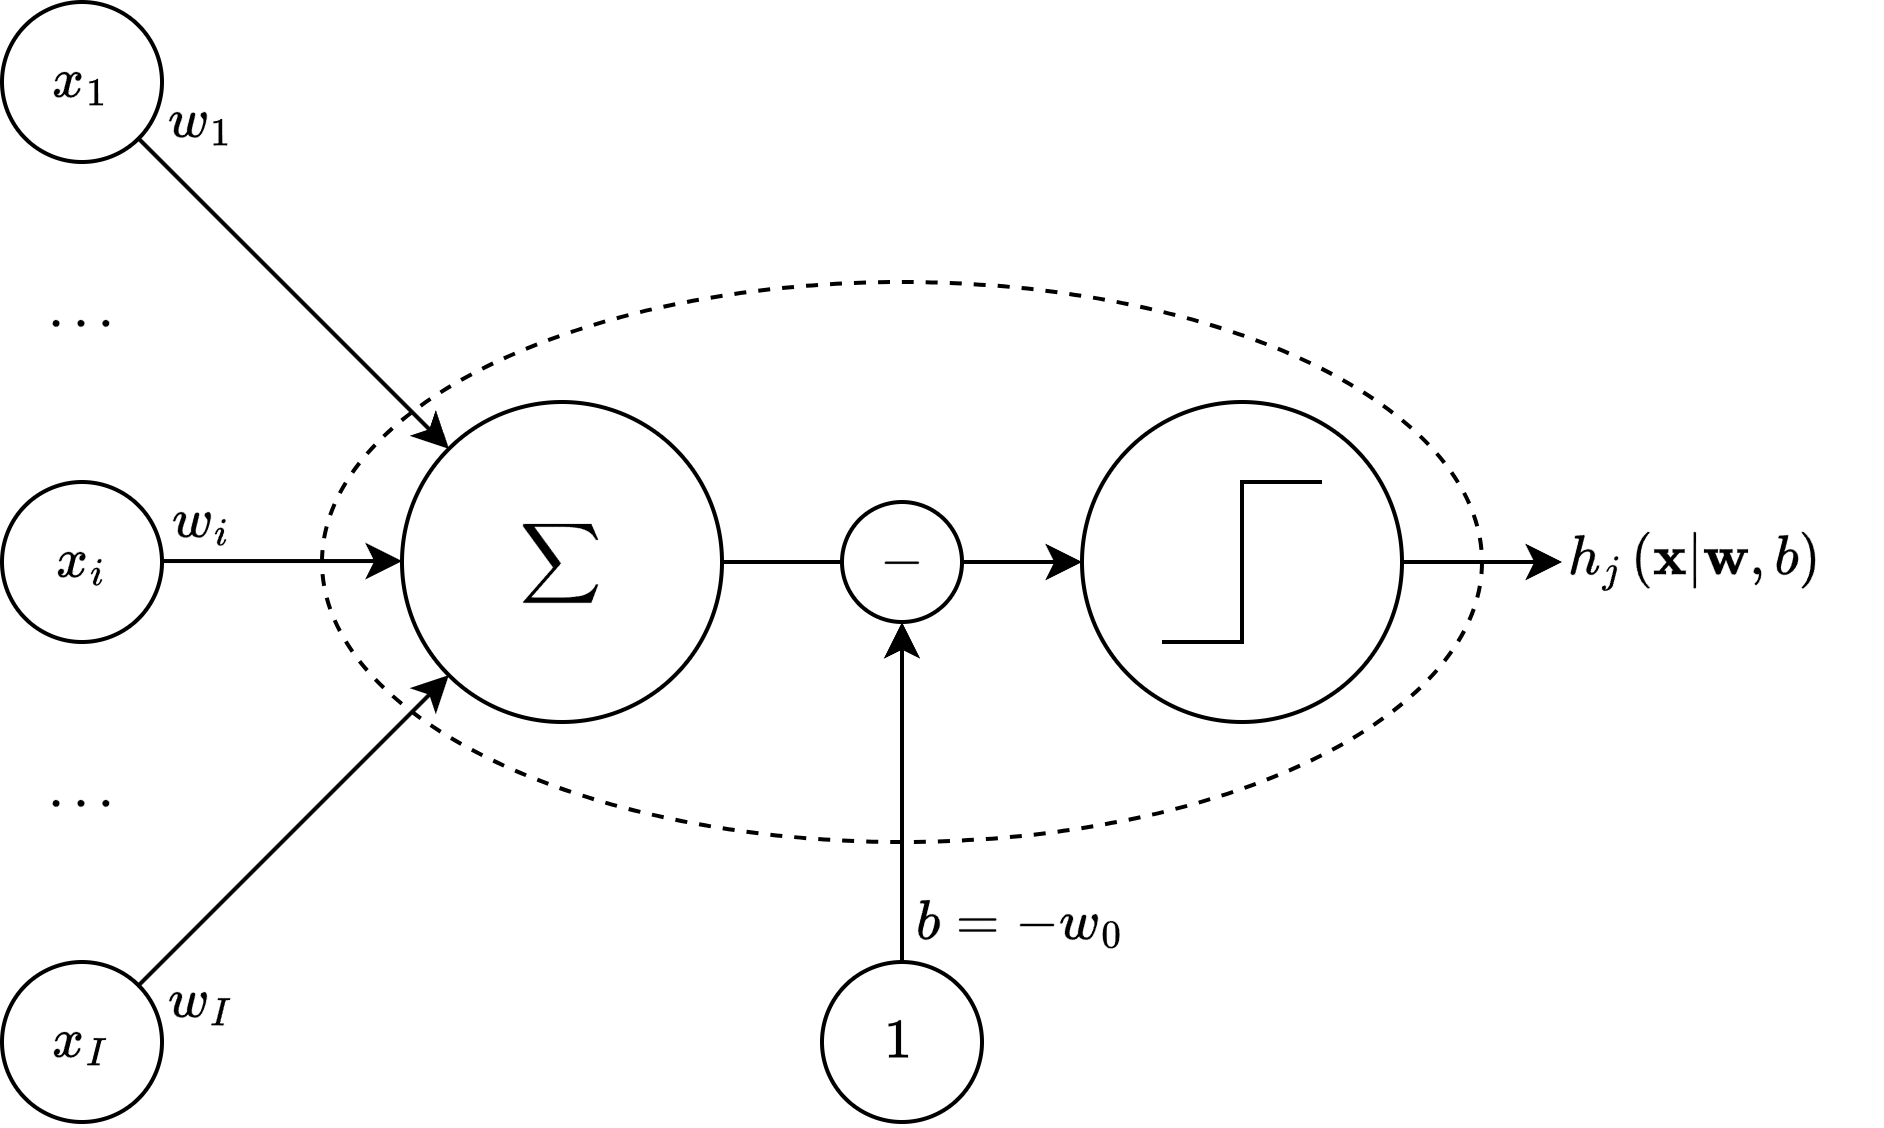
\includegraphics[width=0.75\linewidth]{images/neuron.png}
    \caption{Artificial neuron}
\end{figure}
In this model, the output function $h_j(\mathbf{x}|\mathbf{w},b)$ is defined as:
\[h_j(\mathbf{x}|\mathbf{w},b)=h_j\left(\sum_{i=1}^Iw_ix_i-b\right)=h_j\left(\sum_{i=0}^Iw_ix_i\right)=h_j\left(\mathbf{w}^T\mathbf{x}\right)\]
The function used in an artificial neuron can either be a step function, with values ranging from 0 to 1, or a sine function, with values ranging from -1 to 1.

\paragraph*{History}
Several researchers were actively investigating models for the brain during the mid-20th century. 
In 1943, Warren McCulloch and Walter Pitts proposed the Threshold Logic Unit, also referred to as the Linear Unit, where the activation function was a threshold unit, equivalent to the Heaviside step function. 
A few years later, in 1957, Frank Rosenblatt developed the first Perceptron, with weights encoded in potentiometers, and weight adjustments during learning were performed by electric motors. 
By 1960, Bernard Widrow introduced a significant advancement by representing the threshold value as a bias term in the ADALINE (Adaptive Linear Neuron or later, Adaptive Linear Element). 

\begin{example}
    SLIDE 10
\end{example}

\subsection{Hebbian learning}
The strength of a synapse increases based on the simultaneous activation of the corresponding input and the desired target. 
Hebbian learning can be summarized as follows:
\begin{enumerate}
    \item Begin with a random initialization of the weights.
    \item Adjust the weights for each sample individually (online learning), and only when the sample is not correctly predicted.
\end{enumerate}
Mathematically, this is expressed as:
\[\begin{cases}
    w_i^{k+1}=w_i^k+\Delta w_i^k \\
    \Delta w_i^k=\eta x_i^kt^k
\end{cases}\]
Here, $\eta$ represents the leraning rate, $x_i^k$ is the $i$-th input to  the perceptron at time $k$, and $t^k$ is the desired output at time $k$.

\begin{example}
    SLIDE 12
    we aim to learn the weights necessary to implement the OR operator using a sinusoidal output. 
    We begin with random weights:
    \[\mathbf{w}=\begin{bmatrix} 0 & 0 & 0 \end{bmatrix}\]
    We set the learning rate to $\eta=0.5$. 
    The output function is defined as follows:
    \[h(\mathbf{w}^T\mathbf{x})=\begin{cases}
        1 \qquad\text{ if }\mathbf{w}^T\mathbf{x} > 0 \\
        0 \qquad\text{ if }\mathbf{w}^T\mathbf{x} = 0 \\
        -1 \qquad\text{ if }\mathbf{w}^T\mathbf{x} < 0
    \end{cases}\]
    The process involves cycling through the data records and adjusting the weights for incorrectly classified samples. 
    The learning continues until all records are correctly predicted. 
    In this way, Hebbian learning is applied to achieve the correct implementation of the OR operator.
\end{example}
A perceptron computes a weighted sum and returns the sign (thresholding) of the result:
\[h_j(\mathbf{x}|\mathbf{w})=h_j\left(\sum_{i=0}^Iw_ix_i\right)=\text{Sign}(w_0+w_1x_1+\dots+w_Ix_I)\]
This forms a linear classifier, where the decision boundary is represented by the hyperplane:
\[w_0+w_1x_1+\dots+w_Ix_I=0\]
The linear boundary explains how the perceptron implements Boolean operators. 
However, if the dataset does not have a linearly separable boundary, the perceptron fails to work. 
In such cases, alternative approaches are needed, including non-linear boundaries or different input representations. 
This concept forms the basis for Multi-Layer Perceptrons (MLPs).